% Joint report, DSA4212 group project. DRAFT v4: v3 written as continuous prose (claim first; predictions, explanations and caveats in the text).
% (v1 is report.tex.) Assembled from the two parts:
%   Part A (multimodality): written from multimodality/docs/report_log.md; numbers checked against
%   multimodality/results/summary/.
%   Part B (geometry): condensed from geometry/report/report.tex; numbers from geometry/results/.
% Every section must be rewritten by its author in their own words before submission (see %% AUTHOR notes).
\documentclass[10pt,a4paper]{article}
\usepackage[margin=1.8cm]{geometry}
\usepackage[T1]{fontenc}
\usepackage[utf8]{inputenc}
\usepackage{lmodern}
\usepackage{amsmath,amssymb}
\usepackage{graphicx}
\usepackage{booktabs}
\usepackage{array}
\usepackage{float}   % [H]: keep each part's tables and late figures inside that part
\usepackage[numbers,sort&compress]{natbib}
\usepackage{xcolor}
\usepackage[colorlinks=true,linkcolor=black,citecolor=black,urlcolor=blue]{hyperref}
\setlength{\parskip}{3pt}
\setlength{\parindent}{0pt}
% Compact lists and small captions without extra packages (TinyTeX/Overleaf-safe).
\let\olditemize\itemize
\renewcommand{\itemize}{\olditemize\setlength{\itemsep}{1pt}\setlength{\parskip}{0pt}\setlength{\topsep}{2pt}}
\makeatletter\renewcommand{\@makecaption}[2]{\vskip 4pt{\small\textbf{#1.} #2\par}}\makeatother
\newcommand{\ci}[2]{[#1,\,#2]}
\newcommand{\dec}{\,decades}
\newcolumntype{L}[1]{>{\raggedright\arraybackslash}p{#1}}
\newcommand{\makecell}[1]{\begin{tabular}[c]{@{}c@{}}#1\end{tabular}}  % stand-in for makecell.sty

\title{\vspace{-1.3cm}Does the model fit the landscape?\\
Shape and scale in Bayesian optimisation and CMA-ES\vspace{-0.3cm}}
\author{Isaac Soong Hong Wei (A0272752B), Paul Ng Yin Chen (A0272249Y)\\[2pt]
\small Repository: \url{https://github.com/isaacsoong055/DSA4212}}
\date{\vspace{-0.7cm}}

\begin{document}
\maketitle

\begin{abstract}
\noindent
Bayesian optimisation (BO) and CMA-ES both carry an implicit model of the landscape: CMA-ES a Gaussian
search distribution with a covariance (its shape) and a step size (its scale), BO a Gaussian-process
surrogate whose kernel metric and lengthscales play the same two roles. We test one explanation in two
settings: a method succeeds when its model's shape and scale can match the problem, whatever its family.
\emph{Part A (multimodality)} asks
whether the model's scale lets a method \emph{find} and then \emph{refine} a narrow distant basin: neither
default method finds it; CMA-ES's step size cannot do both jobs at once, and BO succeeds once its lengthscale
is capped (1/50 to 44/50 on fresh seeds) while acquisition tuning helps far less. \emph{Part B (geometry)}
asks whether the model can \emph{tilt}: on rotated, ill-conditioned valleys diagonal CMA-ES, the ARD kernel
and TuRBO's axis-aligned trust region all fail, while their tilting counterparts do not, once BO's own fitting
failures are removed. In both parts the decisive
BO changes were to the model fit, not the acquisition function. All results are in 2-D and pre-registered
predictions are reported whether they held or failed.
\end{abstract}

%=====================================================================
\section{Introduction}
%=====================================================================
%% AUTHORS: joint section, rewrite together in your own words.
\subsection{Motivation and the two methods}
Many optimisation problems give only function values: tuning a model's hyperparameters, calibrating a
simulator, choosing a design. There are no gradients, and each evaluation can cost a training run or a
simulation, so a method must decide where to evaluate next from the values it has seen, and its budget is
counted in evaluations. Bayesian optimisation (BO) and the covariance matrix adaptation evolution strategy
(CMA-ES) are two of the most widely used methods for this setting, and they embody opposite design choices:
BO models the function, while CMA-ES adapts a search distribution.

\emph{BO} \citep{frazier2018tutorial} fits a Gaussian-process (GP) surrogate to all evaluations so far. Its
kernel encodes smoothness and lengthscales, and its posterior gives a prediction and an uncertainty everywhere.
An acquisition function, such as expected improvement (EI), turns these into the next point, trading off
exploiting good predictions against exploring uncertain regions. \emph{CMA-ES} \citep{hansen2016tutorial}
samples a population of $\lambda$ candidates from a Gaussian $\mathcal N(m,\sigma^2C)$, ranks them, moves the
mean towards the best, and adapts the covariance $C$ and the step size $\sigma$ from successful steps. It uses
only the ranking of the values. The basic trade-off follows: BO is sample-efficient because it uses every value
through a global model, but each step is expensive (fitting the GP grows cubically with the number of points)
and its success depends on that model being right; CMA-ES needs more evaluations but each step is nearly free,
and it learns the \emph{local} geometry of the problem.

\subsection{What the literature says, and what it leaves open}
Our questions came from the readings. Hansen's tutorial \citep{hansen2016tutorial} states the invariances
CMA-ES is designed to have: to any order-preserving transformation of $f$, and to rotations and other linear
maps of the search space provided the initial conditions are mapped too; its covariance comes to approximate
the inverse Hessian on a convex quadratic. This raised the question of which invariances survive in practice
and whether a model that cannot rotate pays for it. Restart schemes that grow or mix the population size
(IPOP, BIPOP \citep{auger2005ipop,hansen2009bipop}) were introduced for multimodal functions, which raised the
question of whether population and restarts help find a narrow basin. TuRBO \citep{eriksson2019turbo} restricts
BO's search to local trust regions whose sides are set per coordinate from the ARD lengthscales, an axis-aligned
shape;
COCO \citep{hansen2021coco} sets the benchmarking practice we follow (budgets in evaluations, random instances,
targets and intervals).

The literature also shows that BO's results depend on settings that are rarely reported. Hvarfner et al.
\citep{hvarfner2024vanilla} argue that BO's poor high-dimensional performance owes much to its lengthscale
prior, and that a dimension-scaled prior makes plain BO competitive. Ament et al. \citep{ament2023logei} show
that EI's values and gradients vanish numerically, so the acquisition optimiser can fail; and Siivola et al.
\citep{siivola2018boundary} show that GP-based BO over-explores the boundary of the search box. A comparison of
``BO against CMA-ES'' run with library defaults therefore mixes the family with hidden choices: kernel fitting,
lengthscale bounds, noise handling, step size. What remains open is which of those properties actually
decides success.

\subsection{Problem formulation}
\emph{Research question.} When BO and CMA-ES succeed or fail on a black-box problem, which property of the
method decides the outcome, and does it matter more than the choice of family?

\emph{Guiding hypothesis.} Each method carries an implicit model of the landscape. For CMA-ES it is the search
distribution: the covariance sets its \emph{shape} (orientation and relative stretch) and the step size its
\emph{scale}. For BO it is the GP: the kernel metric sets the shape (a full metric, or the diagonal ARD metric)
and the lengthscales the scale. A method succeeds when its model can match the landscape's shape (orientation,
conditioning) and scale (the size of the features it must find and resolve), and fails when a restriction or a
fitting failure prevents it, whichever family it belongs to.

\subsection{Shared experimental approach}
Both parts fix a budget counted in objective evaluations, with initial designs and restarts included; run
every variant on the same seeds, so comparisons are paired; change one setting at a time against a baseline;
and commit their predictions to the repository before the runs that test them, reporting each as held, partly
held or failed. A method's recommendation is its best evaluated point, judged on the true objective: in Part A
by whether its regret reaches a success threshold, in Part B by its regret in decades of $\log_{10} f$. With
noisy evaluations the recommended point is scored on the noise-free objective, and several recommendation
rules are compared. Uncertainty is given as 95\% intervals: in Part A, Wilson intervals for success rates and
Newcombe intervals for their differences; in Part B, paired bootstrap intervals over instances for differences in
regret, and Wilson intervals for the few success rates it reports. The two parts use different budgets, measures and BO
implementations (BoTorch \citep{balandat2020botorch}; NumPy/SciPy), so their numbers are never put on common
axes.

\subsection{The two directions}
\emph{Part A, multimodality} (Isaac Soong), asks whether each method can \emph{find} a narrow, distant global
basin and then \emph{refine} it, within 300 evaluations. It varies CMA-ES's population size, restarts and step
size, and BO's acquisition function, GP fitting settings and kernel, on a decoy bowl with a narrow Gaussian well
(whose width and distance are varied), with a sphere as a unimodal control and Rastrigin and Schwefel as
validation functions.

\emph{Part B, geometry and parameterisation} (Paul Ng), asks whether a method's model can \emph{tilt} to a
rotated, ill-conditioned valley, and which theoretical invariances survive the implementation. It varies the
conditioning and rotation of the problem and whether each method's model can rotate (full against diagonal
covariance; full against ARD kernel metric; a rotated against an axis-aligned trust region), and also tests
changes of units, monotone transformations of $f$, the box boundary and noisy evaluations, on ellipsoids,
Rosenbrock (COCO f8/f9 \citep{hansen2009bbobfunctions}) and a noisy quadratic, within 200 evaluations.

\subsection{Preview of findings and contributions}
Part A finds that neither default method discovers a narrow, distant basin. For CMA-ES no population size,
restart scheme or step size fixes this, because one step size cannot both find the basin and refine it; for BO,
capping the GP lengthscale does, while tuning the acquisition function helps far less. Part B finds that, in both
families, the version of the method that cannot tilt fails under rotation and the version that can does not; for
BO this became visible only after a fitting failure that stalled every run was diagnosed and fixed, and it then
held across two kernels, two acquisition searches and a TuRBO-style trust region. CMA-ES keeps its rank invariance
exactly; BO keeps neither invariance.

Together the parts contribute a tested account of shape and scale across both families; the shared, unplanned
finding that BO's decisive fixes were to the \emph{model fit}, not to the acquisition function; and a set of
negative and surprising results reported as such: pre-registered predictions that failed, an initial negative
result that turned out to be a fitting failure, a boundary trap, and BO runs that do not repeat bit for bit.

\emph{Roadmap.} Section~\ref{sec:partA} presents Part A and Section~\ref{sec:partB} Part B, each opening with its
answer, then setting out the evidence experiment by experiment, and closing with its predictions against outcomes. Section~\ref{sec:synth} draws the two together and states the limitations.

%=====================================================================
\section{Part A (Multimodality): Can CMA-ES and Bayesian optimisation find a narrow, distant global basin?}\label{sec:partA}
%=====================================================================
%% AUTHOR: Isaac Soong. Replaced from multimodality_section.tex.

\paragraph{Summary.} On a landscape with a wide decoy basin and a narrow, deep global well, neither baseline optimiser reliably finds the well within $N=300$ evaluations (Exp~0: CMA-ES 0 of 50 runs succeed; Bayesian optimisation, BO, 5 of 50). Success was split into \emph{discovery} (a sample lands in the well) and \emph{refinement} (the well is then exploited). For CMA-ES, a larger population and restarts improve discovery but not success, because refinement is limited by the initial step size. For BO, bounding the surrogate's lengthscale raises success from 5/50 to 39/50 (44/50 on fresh seeds); the gain does not carry over to Rastrigin and Schwefel, where the baseline lengthscale never reaches the bound.

%--------------------------------------------------------------
\subsection{Problem and experimental set-up}

\subsubsection{The test landscape}
All method comparisons use one tunable function on $[-5,5]^2$: a wide, shallow \emph{decoy} bowl with a narrow, deep Gaussian \emph{well} cut into it,
\begin{equation}
f(x)=\frac{\lVert x-c\rVert^{2}}{s}-A\exp\!\Big(-\frac{\lVert x-x_g\rVert^{2}}{2w^{2}}\Big),\qquad c=(0,0),\; s=10,\; A=4 .
\end{equation}
The decoy centre $c$ has $f=0$. The well, of width $w$ (default $0.3$), is centred at $x_g=(3,3)$ (\textbf{far}) or $(2,0)$ (\textbf{near}); the global minimum is $f^\ast=-2.208$ (Figure~\ref{fig:land}). The bowl slopes towards $c$ everywhere, so nothing local points to the well. Its width $w$ (how \emph{narrow}) and position (how \emph{distant}) are the two knobs of the study. All distances and widths in this report are in the units of the search box $[-5,5]^2$, which is 10 wide; for example the far well is $\lVert(3,3)\rVert=4.24$ from the decoy centre and the near well is $2$ from it.

\begin{figure}[!ht]
\centering
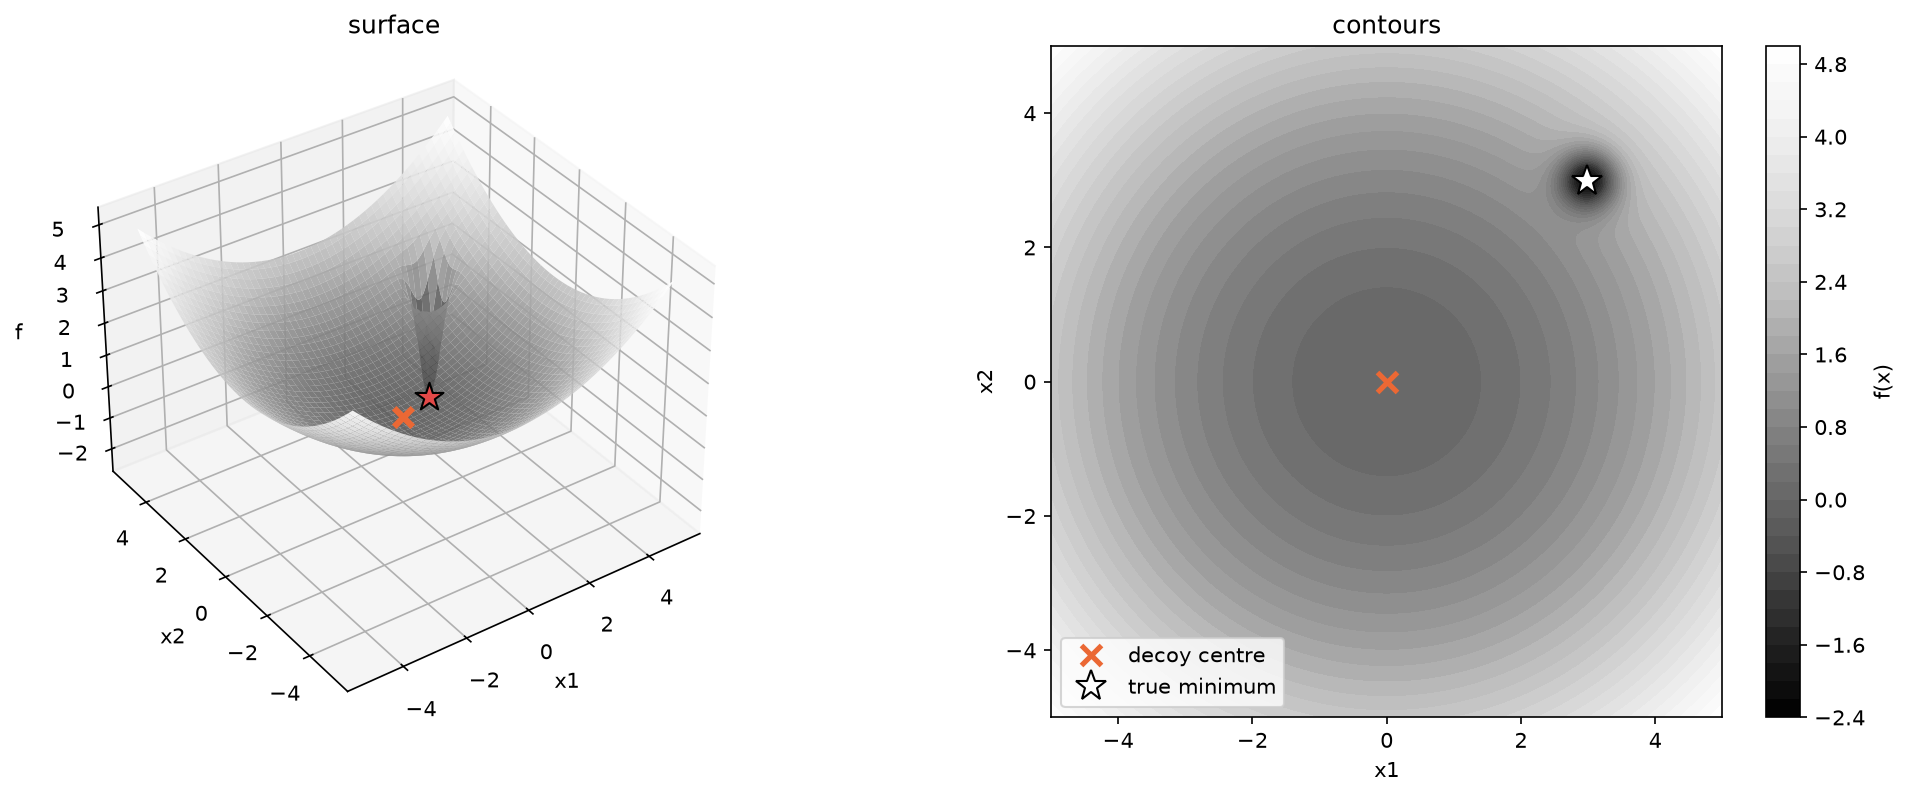
\includegraphics[width=0.42\linewidth]{figures/mm_landscape.png}
\caption{Primary landscape (far well, $w=0.3$): surface (left) and contours (right).}
\label{fig:land}
\end{figure}

\subsubsection{Success criterion}
A run's \emph{regret} is $f(x_{\text{best}})-f^\ast$ for the best point it evaluated. A run \textbf{succeeds} if its regret is at most $\varepsilon=0.05$; otherwise it \textbf{fails}, almost always by converging on the decoy (regret about $2.21$, the well's depth). Success needs two stages, kept apart throughout: \textbf{discovery}, an evaluation within $w$ of the well centre (a \emph{touch}), and \textbf{refinement}, going on from that touch to regret $\le\varepsilon$. The threshold $\varepsilon$ was chosen from random sampling alone: the largest value for which random search with $N=300$ succeeds in at most 5\% of runs. A count $k/50$ is given with a 95\% Wilson interval $[\text{low},\text{high}]$, the range of true success probabilities consistent with $k$ successes in 50 runs; methods are called different only when these intervals, or that of their difference, separate.

\subsubsection{Methods, settings, control and transfer functions}
Table~\ref{tab:settings} gives the baseline of every setting (library default or a value frozen before the large runs) and the experiment that varies it. Exp~0 (the baselines) is the starting point; each later experiment follows from the earlier results and changes exactly one row. Restart triggers were chosen by how often they fire, never by success. The \textbf{sphere} (single basin) is the control: a setting that helps there as well does not owe its gain to multimodality. \textbf{Rastrigin} and \textbf{Schwefel} are \emph{transfer tests} of whether conclusions carry over to standard functions.

\subsubsection{Fair comparison}
Every run uses exactly $N=300$ evaluations, including restarts and BO's initial design (enforced in code), and each experiment uses 50 seeds ($1000,\dots,1049$) on the far well with $w=0.3$, unless marked (the $N=1500$ CMA-ES check, oracle starts, fresh seeds, BO on 20 seeds); these are never compared with BO. One factor changes at a time, on the same seeds. The best variant of each method is re-run on \emph{fresh} seeds $2000,\dots,2049$, so selecting the best of several variants cannot inflate the headline. Baselines were frozen, and the hypotheses committed to the repository (\texttt{predictions.md}, 22 October 2026), before any success rate was seen; later explanations are marked as hypotheses or \emph{post hoc}.

\begin{table}[t]
\centering\footnotesize
\caption{Baseline settings and the experiments that vary them. ``Library'' = software default; ``chosen'' = value fixed before the large runs. BO on the sphere, Rastrigin and Schwefel uses 20 seeds.}
\label{tab:settings}
\footnotesize\begin{tabular}{@{}L{6.1cm}L{3.3cm}L{7.1cm}@{}}
\toprule
Setting (meaning) & Baseline (source) & Varied in \\
\midrule
\multicolumn{3}{@{}l}{\textit{CMA-ES (\texttt{cma} library); Exp 0 = default CMA-ES}} \\
population $\lambda$ (points per generation) & 6 (library) & Exp 1: 12, 24 \\
restarts (fresh start after convergence) & none & Exp 2: IPOP, BIPOP \\
step size $\sigma_0$ (initial spread; box width 10) & 2 (chosen) & Exp 3: 0.3, 0.5, 1, 4 \\
start $x_0$ (initial mean) & $U[-4,4]^2$ (chosen) & Exp 3: ``oracle'' start, mean at distance 1.0 from the well centre \\
\midrule
\multicolumn{3}{@{}l}{\textit{BO (BoTorch); Exp 0 = default BO}} \\
acquisition (next-point rule; $\xi$ = exploration bonus) & EI, $\xi=0$ (standard) & Exps 4, 5: $\xi$ up to 2; LCB; Thompson sampling \\
lengthscale bound (allowed GP lengthscale range) & $[0.05,20]$ (chosen) & Exp 6: upper bound 5, 2, 1, 0.5, 0.25 \\
noise (treats $f$ as noise-free) & fixed $10^{-6}$ (chosen) & Exp 6: $10^{-3}$ to 1; learned; lengthscale prior \\
kernel (GP smoothness) & Mat\'ern-5/2 (BoTorch) & Exp 7: Mat\'ern-3/2, 1/2, RBF (at upper bound 20 and 1) \\
initial design, refit & 10 random points; refit every 5 (chosen) & not varied \\
\midrule
\multicolumn{3}{@{}l}{\textit{Landscape (both methods)}} \\
well (narrowness, distance) & $w=0.3$, far (chosen) & Exp 8: $w\in\{0.1,0.3,0.6,1.0\}$, far and near \\
function & primary landscape & Exp 9: sphere; Exp 10: Rastrigin, Schwefel \\
\bottomrule
\end{tabular}
\end{table}

%--------------------------------------------------------------
\subsection{Results and analysis}\label{sec:results}

\subsubsection{Exp 0: how often do the defaults find the well, and where do they go?}
The intervals overlap, so the methods cannot be told apart at 50 seeds. Almost all runs of both methods end at regret $2.21$: they converged on the decoy.

\begin{table}[!ht]
\centering\footnotesize
\caption{Exp 0 (far well, $w=0.3$, 50 seeds). A touch = an evaluation within $w$ of the well centre.}\label{tab:exp0}
\begin{tabular}{@{}lccccc@{}}
\toprule
Method & Successes & 95\% interval & \makecell{Discovery: runs\\touching the well} & \makecell{Refinement: succ.\\given a touch} & \makecell{Median\\final regret} \\
\midrule
Default CMA-ES & 0/50 & $[0.00,0.07]$ & 1 & 0/1 & 2.21 \\
Default BO (EI, $\xi=0$) & 5/50 & $[0.04,0.21]$ & 5 & 5/5 & 2.21 \\
Random sampling & 2/50 & $[0.01,0.13]$ & -- & -- & 1.11 \\
\bottomrule
\end{tabular}
\end{table}

\textbf{CMA-ES} moves its sampling mean towards the best-ranked points, and step-size adaptation shrinks the spread $\sigma$ once the search has converged \citep{hansen2016tutorial}. In the bowl the best points always lie towards the centre, so $\sigma$ shrinks from 2 to about $10^{-3}$ and from evaluation 100 on at least $97.5\%$ of samples lie within distance $0.5$ of the decoy centre, while the well centre is at distance $4.24$ from it. The one run that touched the well did not refine it: the many decoy samples outweighed the single well sample in the update (Exp~3).

\textbf{BO} fits a Gaussian process (GP) and evaluates next where expected improvement (EI) is largest \citep{frazier2018tutorial,jones1998ego}. The GP's \emph{lengthscale} is how far apart two points must be before the model treats their values as unrelated. In 42 of 50 runs it reached its upper bound of 20, and in all 45 failures no sample entered the well: the model sees one smooth bowl and keeps sampling its centre. So \emph{default BO fails at discovery, not refinement}: all 5 runs that touched the well succeeded (Table~\ref{tab:exp0}). \textbf{Why the maximum lengthscale?} (hypothesis): maximum-likelihood fitting favours smooth explanations \citep{rasmussen2006gpml}, and for near-noise-free data that look like a smooth trend the estimate can grow without limit \citep{karvonen2022illposed}; here the noise is fixed at $10^{-6}$ and the data are an exact bowl.

\subsubsection{Exps 1--3: CMA-ES}
\textbf{Observation:} in Exp~0, CMA-ES converged on the decoy; only 1 of 50 runs touched the well, and it did not refine it. Hypotheses A and B act on discovery, C on refinement.

\textbf{Hypothesis A: a larger population finds the well more often and succeeds more (Exp 1).} More points per generation should put more early samples in the well \citep{hansen2016tutorial}. \emph{Test:} $\lambda\in\{6,12,24\}$. \emph{Result} (Table~\ref{tab:cma12}): discovery improved (touches: 1, 7, 13 of 50 runs) but refinement did not (successes given a touch: 0/1, 0/7, 0/13). Since $\lambda=24$ allows only 13 generations, a follow-up experiment with $N=1500$ checked whether the failure was caused by this cut-off; it again gave 0/50. \emph{Answer:} a larger population improves discovery, not success. \emph{Why (tested in Exp~3):} a larger $\lambda$ adds samples but leaves the spread $\sigma_0=2\gg w$ unchanged, so the many decoy samples still outweigh a well sample in the update.

\textbf{Hypothesis B: restarts help (Exp 2).} Restarting after convergence, with larger populations (IPOP \citep{auger2005ipop}) or a mix of large and small (BIPOP \citep{hansen2009bipop}), gives fresh chances to land in the well. \emph{Result:} 0/50 for none, IPOP and BIPOP (identical here: only one restart fits in 300 evaluations); the well was touched in 6 runs, like a fresh $\lambda=12$ start (7). \emph{Answer:} no; a restart is a new attempt with the same small chance.

\begin{table}[!ht]
\centering\footnotesize
\caption{Exps 1, 2: every setting gives 0/50 successes (interval $[0.00,0.07]$).}\label{tab:cma12}
\begin{tabular}{@{}lccc@{}}
\toprule
Setting & Successes & Runs with a sample in the well & Median generations \\
\midrule
$\lambda=6$ (default) & 0/50 & 1 & 50 \\
$\lambda=12$ & 0/50 & 7 & 25 \\
$\lambda=24$ & 0/50 & 13 & 13 \\
IPOP / BIPOP (identical) & 0/50 & 6 & -- \\
\bottomrule
\end{tabular}
\end{table}

\textbf{Hypothesis C: the step size is too large to refine a narrow well (Exp 3).} With $\sigma_0=2\gg w=0.3$, the many selected decoy points can outweigh one well sample. \emph{Test:} vary $\sigma_0$ from the usual random start (success = finding \emph{and} refining) and from an ``oracle'' start whose initial mean is at distance 1.0 from the well centre (success = refining alone). \emph{Result} (Table~\ref{tab:sig}): from the random start no setting exceeds 1/50; from the oracle start success falls from 33/50 at $\sigma_0=0.3$ to 2/50 at the default $2$. With $\sigma_0=2$ the search mean drifts within about five generations to the decoy centre; with $\sigma_0=0.3$ it converges onto the well. Finding and refining pull $\sigma_0$ in opposite directions: a small $\sigma_0$ refines a nearby well but never reaches a distant one; a large one touches it more but cannot exploit it. \emph{Answer:} yes; this is why $\lambda$ and restarts, which only affect touching, left success unchanged.

\emph{Follow-up to Exp~3 (does only the ratio $\sigma_0/w$ matter?).} Here the initial step size is $\sigma_0=kw$, a multiple $k=1,3,7,20$ of the well width, tested at $w=0.1$ to $1.0$, from an oracle start at distance $10w/3$ from the well centre (50 seeds each). Narrow wells repeat Exp~3 (at $w=0.1$: 44/50 for $k=1$, 0/50 for $k=20$), but at $w=1.0$ it reverses: 24/50 for $k=1$, 40/50 for $k=20$. Success is therefore not a function of $\sigma_0/w$ alone; a wide well is found by a broad cloud. The \texttt{cma} library caps the step size at about 4 in this box, so $k=7$ and $20$ coincide for $w\ge0.6$; Exp~3 ($\sigma_0\le4$) is unaffected.

\begin{table}[!ht]
\centering\footnotesize
\caption{Exp 3: successes out of 50 (touches in brackets).}\label{tab:sig}
\begin{tabular}{@{}lccccc@{}}
\toprule
$\sigma_0$ & 0.3 & 0.5 & 1 & 2 (default) & 4 \\
\midrule
Random start & 0 (0) & 0 (0) & 1 (2) & 0 (1) & 0 (4) \\
Oracle start & 33 (35) & 31 (39) & 10 (23) & 2 (11) & 1 (11) \\
\bottomrule
\end{tabular}
\end{table}

\subsubsection{Exps 4--7: BO}
\textbf{Observation:} default BO fails at discovery.

\textbf{Hypothesis D: more exploration helps (Exps 4, 5).} \emph{Test:} raise EI's exploration parameter $\xi$ (a bonus on uncertain points); replace EI by the lower confidence bound (LCB) or Thompson sampling. \emph{Result} (successes out of 50): moderate exploration helps a little ($\xi=0.1$: 17/50, $+0.24$, interval $[+0.08,+0.39]$), too much hurts ($\xi=0.01,0.5,1,2$: 8, 12, 5, 3), and LCB (3--4/50) and Thompson sampling (3/50) do not help. With large $\xi$ the well is found late and successes given a touch fall from 17/45 at $\xi=0.1$ to 3/42 at $\xi=2$; why late finds are exploited poorly is unresolved. \emph{Answer:} more exploration helps only modestly: the best setting ($\xi=0.1$) lifts success from 5/50 to 17/50, and further increases make it worse.

\textbf{Hypothesis E: the fitted lengthscale is the limit (Exp 6).} Exploration tuning gave at most 17/50, while the lengthscale sat at its bound in 42/50 runs. \emph{Test:} lower the upper bound to 5, 2, 1, 0.5, 0.25 (one value per arm); separately, change the noise level and add BoTorch's lengthscale prior. \emph{Result} (Table~\ref{tab:cap}): a bound of 1 (about $3w$) gives 39/50, $+0.68$ over the default (interval $[+0.51,+0.79]$), the most effective change in the study. A smaller bound makes distant points unrelated, so EI keeps sampling unexplored regions (about 100 distinct $1\times1$ cells with bound 1, against 10) and a sampled well is exploited. A bound of 0.25 ($\approx w$), noise settings and a soft prior do not help (at most 6/50). \emph{Answer:} yes; a hard bound on the lengthscale is what matters.

\begin{table}[!ht]
\centering\footnotesize
\caption{Exp 6: upper bound on the BO lengthscale; difference vs the default (bound 20).}\label{tab:cap}
\begin{tabular}{@{}lcccccc@{}}
\toprule
Bound & 20 (default) & 5 & 2 & 1 & 0.5 & 0.25 \\
\midrule
Successes & 5/50 & 11/50 & 28/50 & \textbf{39/50} & 22/50 & 6/50 \\
95\% interval & $[0.04,0.21]$ & $[0.13,0.35]$ & $[0.42,0.69]$ & $[0.65,0.87]$ & $[0.31,0.58]$ & $[0.06,0.24]$ \\
Difference & -- & $+0.12$ & $+0.46$ & $+0.68$ & $+0.34$ & $+0.02$ \\
Runs touching the well & 5 & 12 & 29 & 41 & 24 & 6 \\
\bottomrule
\end{tabular}
\end{table}

\textbf{Hypothesis F: the gain depends on the kernel (Exp 7).} With the lengthscale upper bound at 20 no kernel differs from Mat\'ern-5/2 (5/50). With the upper bound at 1 the rougher Mat\'ern-3/2 and 1/2 drop to 6/50 and 3/50, while RBF matches Mat\'ern-5/2 (39/50). A likely reason (hypothesis, from the kernel formulas \citep{rasmussen2006gpml}): the same lengthscale gives a different correlation range. At a distance equal to the lengthscale the correlation is $0.37$ (Mat\'ern-1/2), $0.48$ (3/2), $0.52$ (5/2) and $0.61$ (RBF), so with the bound at 1 the rough kernels behave as if it were tighter, and they rarely touch the well (6 and 3 runs, against 41). Testing this needs a separate bound per kernel. \emph{Answer:} yes, for the rougher kernels.

\subsubsection{Exp 8: headline result across well widths}
\emph{Test:} $w\in\{0.1,0.3,0.6,1.0\}$ for the far well and $w\in\{0.1,0.3\}$ for the near well (at $w\ge0.6$ it merges with the bowl). Defaults use seeds 1000--1049; the best variant of each method (CMA-ES $\sigma_0=1$, chosen on 1/50; BO bound 1) is re-run on fresh seeds (Figure~\ref{fig:width}).

\begin{figure}[!ht]
\centering
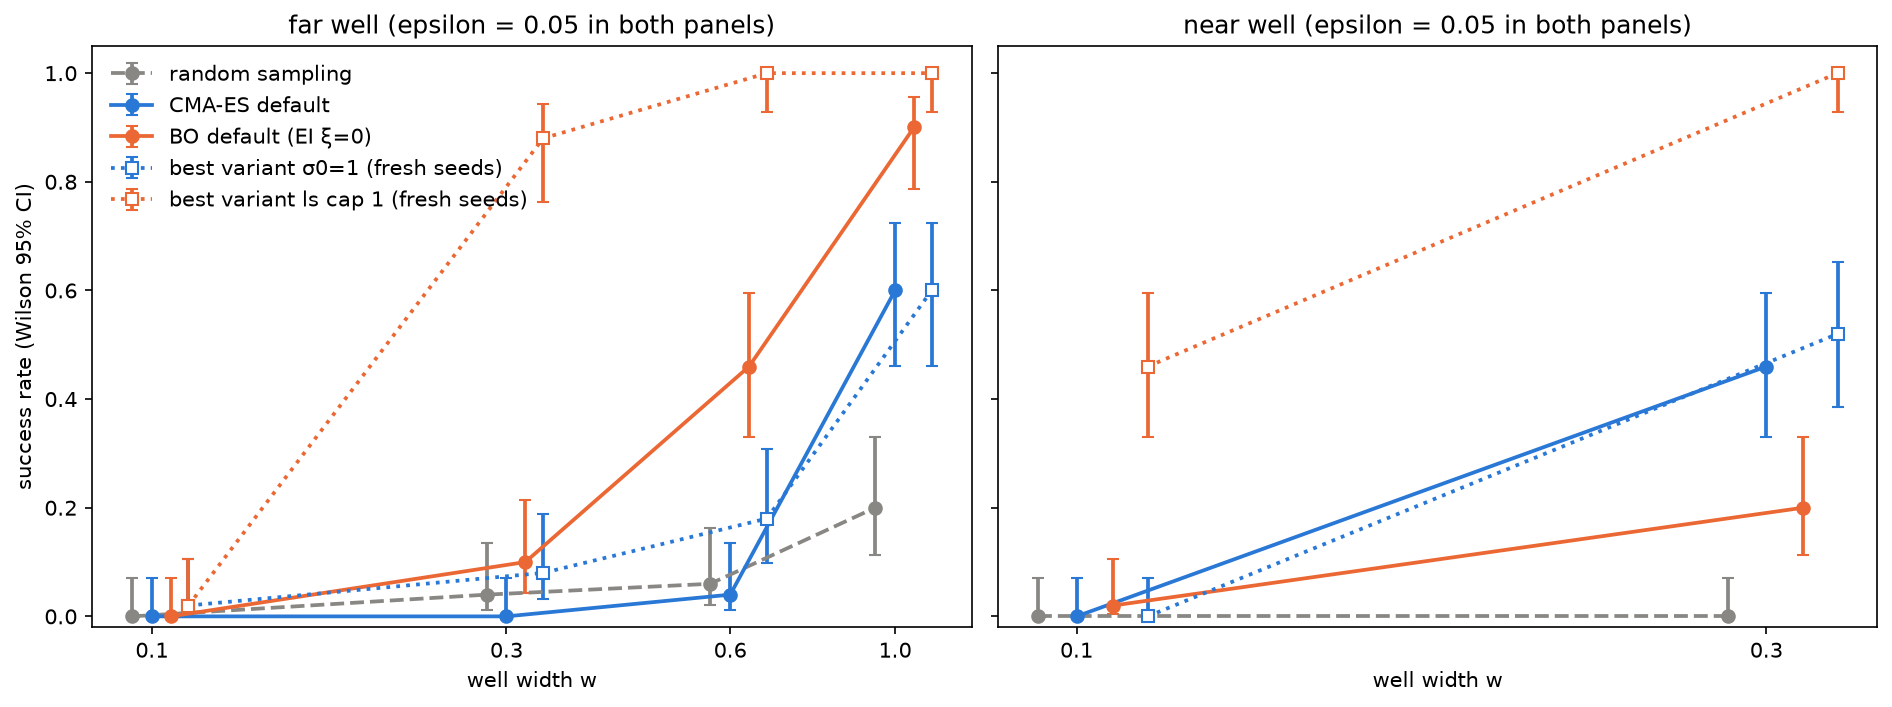
\includegraphics[width=0.58\linewidth]{figures/mm_exp8_width.png}
\caption{Exp 8: success rate against $w$ for the far well (left) and the near well (right); Wilson 95\% intervals, successes out of 50 printed. Solid: defaults (seeds 1000--1049); dotted: best variants (fresh seeds 2000--2049).}\label{fig:width}
\end{figure}

\textbf{Width.} Success rises with $w$ for every method (default CMA-ES: 0/50 at $w=0.3$, 30/50 at $w=1.0$). The main reason is the size of the target: the well's catchment is a disc of radius $w$, so 300 random points in the $10\times10$ box touch it about $300\pi w^2/100=0.1,\,0.8,\,3.4,\,9.4$ times for $w=0.1,\,0.3,\,0.6,\,1.0$, matching random search (0, 2, 3, 10 of 50 successes); a wide well is also easier for a broad cloud or a GP to notice. BO with bound 1 reaches 44/50 at $w=0.3$ on fresh seeds (39/50 on the selection seeds) and 50/50 at $w=0.6$ and $1.0$, but only 1/50 at $w=0.1$: even the bounded model rarely samples so narrow a well. CMA-ES with $\sigma_0=1$ shows no gain at any width.

\textbf{Distance.} On the \emph{near} well, default CMA-ES beats default BO at $w=0.3$ (23/50 and 30/50 on the two seed sets, against 10/50 and 13/50), whereas on the far well it does not. A likely reason (hypothesis): the near well lies at distance 2 from the decoy centre (the far well: 4.24), so CMA-ES's initial cloud (spread $\sigma_0=2$) and the mean's path to the centre pass close to it. Unexplained: default BO at $w=0.6$ scores 23/50 on seeds 1000--1049 but 10/50 on fresh seeds.

\subsubsection{Exps 9--10: control and transfer}
\textbf{Sphere (control).} Every setting succeeds in every run: the sphere has one basin, and the success threshold $\varepsilon=0.05$ is far above every final regret. The settings differ only in \emph{precision}: a larger population gives a \emph{worse} final regret (median $1.6\times10^{-10}$, $9.8\times10^{-8}$, $6.0\times10^{-5}$ for $\lambda=6,12,24$). The cause is the fixed budget: on a single smooth basin CMA-ES shrinks its regret by a roughly constant factor per generation, so precision is set by the number of generations, and $N=300$ allows only 50, 25 and 13 for $\lambda=6,12,24$. A bigger population takes a slightly better step (it averages over more points), but that does not make up for the lost steps.

\textbf{Rastrigin and Schwefel (transfer).} The bound's large gain does \emph{not} carry over cleanly (Table~\ref{tab:valid}). Success rises with the bound on both functions, $+0.10$ on Rastrigin (interval $[-0.19,+0.37]$) and $+0.20$ on Schwefel ($[-0.0003,+0.42]$), but with 20 seeds neither can be separated from zero, and BO already scores 16/20 on Schwefel, so 20/20 is the ceiling. CMA-ES population size has no distinguishable effect. The logged fits show where the bound can act (post hoc; last column of Table~\ref{tab:valid}). On the sphere and the primary landscape it is 8--9 after the initial design and ends at the bound of 20 (20 of 20 and 86 of 100 runs). On Rastrigin it falls from 1.3 to $0.41$, shorter than the function's period of 1: it ends below 1 in all 20 runs, so a bound of 1 can only act early. On Schwefel the median rises from $0.56$ to $1.28$ and ends above 1 in 14 of 20 runs, so a bound of 1 \emph{is} active there, which fits its small increase. Neither function reaches the bound of 20. A likely reason (hypothesis): the sphere and primary landscape are a smooth bowl, which a long lengthscale fits best, whereas Rastrigin and Schwefel oscillate over distances of about 1. This gives a rule: \emph{the large gain needs the baseline lengthscale to run to its maximum and a narrow basin to be hidden.} The primary landscape meets both; the sphere only the first (and the bound costs accuracy there); Rastrigin and Schwefel neither, so the bound is inactive or mildly active and the gain small and uncertain.

\textbf{What follows.} A bound should not be applied blindly: first check whether the fitted lengthscale sits at its upper limit, then bound it, at a few well widths. Confirming the rule needs a per-function bound (e.g.\ below 0.4 on Rastrigin) or more seeds. BO also beats CMA-ES on Schwefel (16/20 against 2--8 of 50), unexpectedly; no bug or configuration slip was found.

\begin{table}[!ht]
\centering\footnotesize
\caption{Exp 10: successes (CMA-ES, random: 50 seeds; BO: 20); $\varepsilon=0.2$ (Rastrigin), $5.0$ (Schwefel). Last column: median fitted lengthscale of default BO (box units, upper bound 20) after the initial design $\to$ at the end of the run (logged fits).}\label{tab:valid}
\begin{tabular}{@{}lcccccccc@{}}
\toprule
 & \makecell{CMA-ES\\$\lambda=6$} & $\lambda=12$ & $\lambda=24$ & $\sigma_0=1$ & \makecell{BO\\default} & \makecell{BO\\bound 1} & Random & \makecell{BO default\\lengthscale} \\
\midrule
Rastrigin & 8/50 & 11/50 & 4/50 & 7/50 & 8/20 & 10/20 & 1/50 & $1.29\to0.41$ \\
Schwefel & 8/50 & 6/50 & 2/50 & 4/50 & 16/20 & 20/20 & 2/50 & $0.56\to1.28$ \\
\bottomrule
\end{tabular}
\end{table}

%--------------------------------------------------------------
\subsection{Limitations}
\begin{itemize}
\item \textbf{Scope and selection.} One main landscape in two dimensions with one $\varepsilon$; the Rastrigin and Schwefel explanation rests on four landscapes and 20 BO seeds, too few to separate $+0.20$ on Schwefel from zero. Bound 1 is the best of five values, so 39/50 is optimistic (44/50 on fresh seeds); 50 seeds give intervals of about $\pm14$ points.
\item \textbf{Frozen settings and mechanisms.} The BO failure depends on the chosen bound of 20; the explanations for the maximal lengthscale, late finds, kernels and the near well are hypotheses.
\end{itemize}

\subsection{Conclusion}
At a fixed budget of 300 evaluations, both baselines fail on a narrow, distant well because they never \emph{find} it. For CMA-ES, a larger population and restarts only add chances to touch it, and a small step refines only a nearby well. For BO, bounding the lengthscale at about three well widths turned 5/50 into 39/50, provided the baseline lengthscale runs to its upper limit.

% Smaller headings from Part B onwards (section: large, subsection: normalsize).
\makeatletter
\renewcommand\section{\@startsection{section}{1}{\z@}{-3.5ex \@plus -1ex \@minus -.2ex}{2.3ex \@plus.2ex}{\normalfont\large\bfseries}}
\renewcommand\subsection{\@startsection{subsection}{2}{\z@}{-3.25ex\@plus -1ex \@minus -.2ex}{1.5ex \@plus .2ex}{\normalfont\normalsize\bfseries}}
\makeatother

%=====================================================================
\section{Part B: can the search tilt? (geometry and parameterisation)}\label{sec:partB}
%=====================================================================
%% AUTHOR: Paul Ng. Condensed from geometry/report/report.tex; rewrite in your own words.
\emph{Answer in brief.} In both families, the version of the method that cannot tilt fails under rotation and the
version that can does not; for BO this became visible only after a fitting failure was found and fixed. CMA-ES keeps
its rank invariance exactly; BO keeps neither invariance, and its behaviour at the box edge and under noise depends
on implementation details.

\subsection{Question, set-up and predictions}
Near a minimum $f\approx f^*+\tfrac12h^\top Hh$. The Hessian's eigenvalues
are the curvatures; their ratio $\kappa$ is the conditioning (a narrow valley when large); its eigenvectors
are the valley's orientation, which a rotation changes without changing $\kappa$. A full covariance
(CMA-ES) or a full kernel metric $M=LL^\top$ (BO) can align with a rotated valley; a diagonal covariance,
the standard ARD kernel and TuRBO's axis-aligned trust region \citep{eriksson2019turbo} cannot. We predicted
that (i) each axis-restricted method pays a penalty under rotation that its tilting counterpart does not,
(ii) only when the problem is both ill-conditioned and rotated, and (iii) the tilting version pays a small
price when no tilt is needed.

2-D ellipsoids with log-spaced eigenvalues from 1 to $\kappa$, the optimum on a radius-2
sphere, aligned or Haar-rotated, 15 instances (COCO-style; seed = instance). CMA-ES follows Hansen's
tutorial, with a diagonal ablation. BO is GP-EI (initial design of $2d+4$, EI over 200 uniform candidates
polished by L-BFGS-B, targets log-transformed) with a MAP lengthscale prior on the metric's
eigen-lengthscales \citep{hvarfner2024vanilla}, so that the prior does not favour axis-aligned metrics. Both
get the box $[-5,5]^2$ (BO searches it; CMA-ES starts at its centre with $\sigma_0=3$) and 200 evaluations. We report regret
after that fixed budget because BO cannot run much longer (each run takes minutes), and give the runtime to a target,
the measure COCO recommends \citep{hansen2021coco}, where the two views differ.

\subsection{CMA-ES fails under rotation only when it cannot tilt (E1, E7)}
Diagonal CMA-ES fails on a rotated, ill-conditioned valley and full CMA-ES does not, as predictions (i) and (ii) require. At
$\kappa=1{,}000$ diagonal CMA-ES solves every instance at $0^\circ$ and $90^\circ$ and none between $30^\circ$ and $60^\circ$ (0/15 at each, \ci{0}{0.20}), while full
CMA-ES solves every angle (Fig.~\ref{fig:e1}); at $\kappa=100$ both succeed everywhere. The $90^\circ$ control only swaps the axes and
recovers fully, so the rotation, not the conditioning, causes the failure. Full CMA-ES is rotation-invariant in distribution (405
against 408 median evaluations under Haar rotation).
IPOP-style restarts leave the diagonal failure in place (1/15 against 3/15 reaching $10^{-5}$ at rotated $\kappa=10^4$; difference $-0.13$ \ci{-0.39}{+0.13}, not significant), since a
restarted diagonal run still cannot tilt. These runs use 4,000 evaluations, longer than the 200-evaluation head-to-head.
E1 starts at $(2,\dots,2)$ with $\sigma_0=2$ and counts a run as solved at $f\le10^{-8}$; E7 starts at the box
centre with $\sigma_0=3$, as in the head-to-head.

\begin{figure}[t]
\centering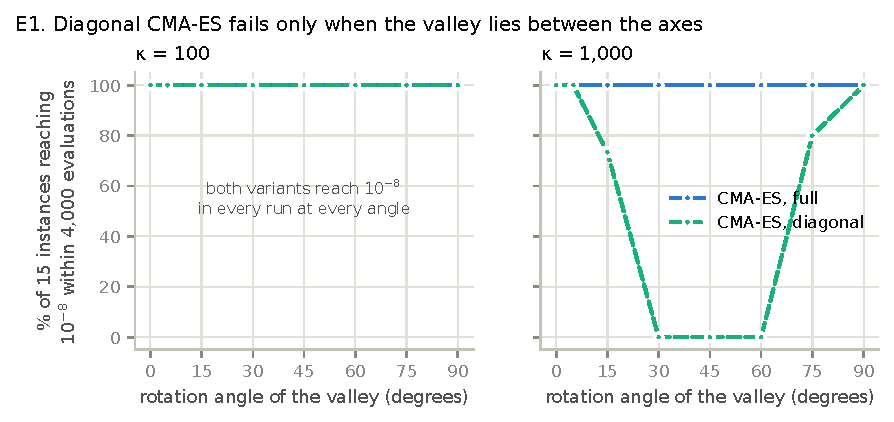
\includegraphics[width=0.78\linewidth]{figures/geom_e1_angle.pdf}
\caption{Part B, E1. Success of full (solid) and diagonal (dashed) CMA-ES against the angle of a 2-D valley.}
\label{fig:e1}
\end{figure}

\subsection{BO first showed no penalty, because a fitting failure stalled every run (E2, E2e)}\label{sec:stall}
BO's first head-to-head contradicted prediction (i), and the cause was a fitting failure, not the geometry. ARD's learned long
axis is off by exactly $45^\circ$ on $45^\circ$ problems, while the full metric is within $0.2^\circ$--$4^\circ$, so ARD cannot tilt;
yet its rotation penalty was $+0.05$ \ci{-0.53}{+0.63} decades at $\kappa=100$, while diagonal CMA-ES paid $+1.70$ \ci{+0.41}{+2.57}.
BO was stalling near $10^{-2.6}$ even on the round bowl. Per-iteration logs ruled out the target transform's floor and the candidate
search, and showed the GP fitting a noise term (SD 0.2--0.4) to a noise-free function: it explained its best points away as noise, its
prediction at the incumbent sat 2--2.5 times the gap to the second-best point above the observed value, and EI underflowed below
$10^{-12}$ in 97--100\% of late iterations. BO fits the GP to $\log f$, because raw values on these problems span many orders of magnitude and would
otherwise be dominated by the few largest. But the log turns the optimum into a sharp dip. The GP's
lengthscales (one per direction, with ARD) are the same everywhere in the box, so following the dip would make
its whole surface wiggly; since it also learns its noise level, it finds it cheaper to call the dip noise.
Each of the three is needed: fixing the noise removes the way out (the fix below), dropping the log removes the
dip, and a kernel whose lengthscales vary with location (non-stationary) would let the GP bend only near the
optimum. We tested only the first; a locally fitted GP, a crude form of the third, lost for lack of data (E12, Section~\ref{sec:bend}). Fixing the noise variance at $10^{-6}$ lifted BO by $-1.17$ \ci{-1.71}{-0.74} decades,
whereas LogEI \citep{ament2023logei}, which fixes the underflow but not its cause, changed nothing ($+0.01$ \ci{-0.79}{+0.47}). For a deterministic objective the noise should be fixed near zero; we had kept the usual default (as in
BoTorch) of learning it, and E2e shows how that default fails here. Section~\ref{sec:noise} tests the fix under noise.

\subsection{Once BO works, the axis-restricted version pays in every variant (E2, E8, E10)}\label{sec:bowork}
With the fix, BO-ARD pays a rotation penalty and BO-full does not, as predictions (i) and (ii) require, across two kernels, two
acquisition searches and a trust region. Run on one machine, BO-ARD's penalty became $+2.01$ \ci{+1.28}{+2.97} decades at
$\kappa=10^4$ and BO-full's stayed non-significant (Fig.~\ref{fig:pen}). Table~\ref{tab:robust} repeats the comparison with a
Mat\'ern-5/2 kernel, 200 extra candidates around the incumbent, and a TuRBO-style trust region \citep{eriksson2019turbo} whose box is
either axis-aligned with ARD-scaled sides or rotated to the full metric; in every variant the axis-restricted version ends
significantly behind on rotated problems. The reason is shared: the ARD kernel and the published trust region both scale each
coordinate separately, so neither can align with a rotated valley. Measured by runtime to a target, BO's standing depends on its search:
on the round bowl CMA-ES reaches $10^{-5}$ in every run (median 142--154 evaluations), BO with the noise fix in only 0--4 of 15 runs (at most \ci{0.11}{0.52})
within 200, and BO with local candidates in every run (median 41--56). Across families, the trust region suited to each problem beats full CMA-ES at 200
evaluations: the axis-aligned box on aligned $\kappa=100$ ($-1.36$ \ci{-2.02}{-0.85}) and the rotated box on rotated
$\kappa=10^4$ ($-3.32$ \ci{-4.24}{-1.82}; the axis-aligned box there: $-0.41$ \ci{-1.24}{+0.24}), while with plain
EI CMA-ES wins by 200 evaluations at $\kappa\le100$. Since long BO runs are not bit-repeatable, these results hold in distribution; the
wide aligned intervals in Table~\ref{tab:robust} come from the boundary trap (Section~\ref{sec:boundary}).

\begin{figure}[t]
\centering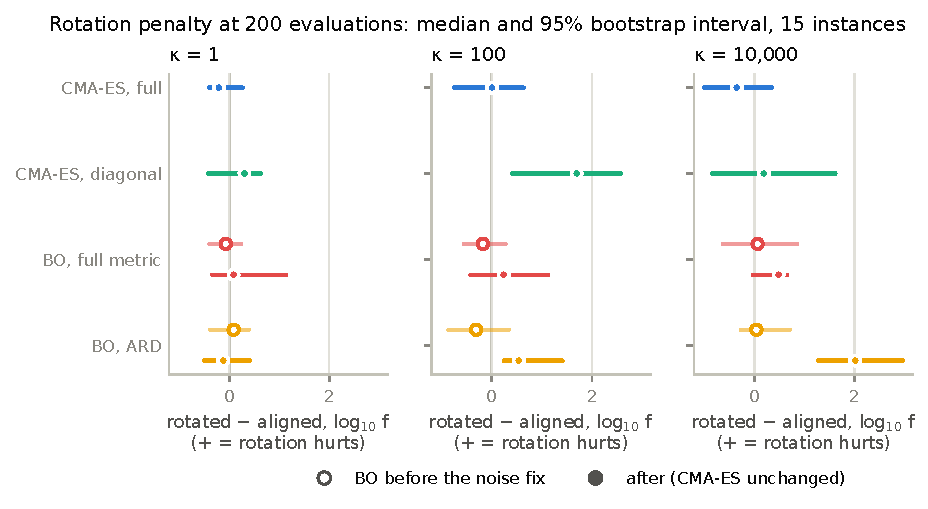
\includegraphics[width=0.86\linewidth]{figures/geom_rotation_penalty.pdf}
\caption{Part B. Rotation penalty at 200 evaluations (median, 95\% bootstrap interval, 15 instances). Hollow: BO
before the noise fix. The axis-restricted variant pays in both families once BO is no longer stalled.}
\label{fig:pen}
\end{figure}

\begin{table}[t]
\centering\small
\begin{tabular}{lcc}
\toprule
BO variant (2-D, 15 instances, 200 evaluations) & rotated $\kappa=10^4$ & aligned $\kappa=10^4$ \\
\midrule
EI, squared exponential, noise fixed & $+1.40$ \ci{+0.68}{+1.69} & $-0.13$ \ci{-1.15}{+0.19} \\
EI, Mat\'ern-5/2 & $+1.06$ \ci{+0.59}{+1.43} & $-0.13$ \ci{-0.70}{+0.54} \\
EI + local candidates & $+1.28$ \ci{+0.12}{+2.36} & $-2.96$ \ci{-3.44}{+2.61} \\
Trust region, ARD box vs rotated box & $+2.92$ \ci{+1.27}{+3.79} & $-0.39$ \ci{-3.11}{+4.65} \\
\bottomrule
\end{tabular}
\caption{Part B. Axis-restricted minus tilting version, median $\log_{10}f$ at 200 evaluations, paired by instance
(+ = axis-restricted worse). Wide aligned intervals come from the boundary trap.}
\label{tab:robust}
\end{table}

\subsection{On a bending valley, local orientation and local search decide (E5, E9, E12)}\label{sec:bend}
On Rosenbrock, whose valley bends, what matters is the local orientation, and for BO local \emph{search} helps while a locally
\emph{fitted} model does not; both of our predictions here failed. We expected both CMA-ES variants to converge given 4,000
evaluations, but only full CMA-ES did, reaching $10^{-5}$ in every run (median about 500 evaluations), while diagonal did so in 0/15
(f8; \ci{0}{0.20}) and 4/15 (f9; \ci{0.11}{0.52}) runs. The reason is that even ``aligned'' Rosenbrock is tilted $63.5^\circ$ near its optimum (local
$\kappa\approx2{,}500$), so no fixed axis alignment fits it. For BO at 300 evaluations, the trust region beats plain BO by 3.5--3.7
decades and its tilted box beats the axis-aligned one by 2.0--2.5 decades, even on f8. Plain BO's kernel adapts its lengthscales but
is stationary, one metric for the whole box, which can only average the directions along a curving valley, whereas inside a small box
the valley is close to a straight, tilted one. We also expected a trust region whose GP is fitted only to the points inside it (at
least 20), rather than to all points since its last restart as in the ordinary trust region, with the search
unchanged, to follow the bend better; instead it trailed the ordinary trust region by 1.8--2.0 decades, though it stayed about 1.7
ahead of plain BO. A quadratic control, where the shape is the same everywhere and a local fit can gain nothing, shows why: there
local fitting lost 2.7 decades, so its loss comes from fitting fewer points, not from geometry. TuRBO's authors found the opposite,
that local GPs predicted better than a global GP on a 14-D robot-pushing problem with 200 points per region and an objective whose
noise and lengthscales vary by region \citep[Sec.~3.6]{eriksson2019turbo}. We suggest, but have not tested, that local fitting pays
when each region holds enough data and the function really differs between regions, which neither our 2-D runs nor our smooth
valley provide. Part of the trust region's lead may also come from its denser local search, 1,000 candidates inside its box against
plain BO's 200 across the whole box, which this experiment does not separate.

\subsection{CMA-ES keeps its invariances when set up as the theory requires; BO keeps neither (E3)}\label{sec:invariance}
CMA-ES is designed to be invariant to strictly increasing transformations of $f$ (it uses only rankings) and
to invertible linear maps of the search space, provided its initial mean and covariance are mapped too
\citep{hansen2016tutorial}; BO has neither property by design. We tested both on the aligned $\kappa=100$
quadratic, scoring every run on the original $f$ and pairing it with an unchanged baseline.

\emph{Monotone transformations of $f$.} Under $\log(1+f)$, $f^3$, $\sqrt f$ and $f+1$, both CMA-ES variants
produced runs bit-identical to the baseline in all 120 cases (their one use of an $f$ value, the stopping
target, was set to 0, which no run reaches). BO was not invariant, and the direction depends
on the transformation: cubing $f$ cost 1.7 decades ($+1.72$ \ci{+1.14}{+2.22} for ARD), while $\log(1+f)$
and $f+1$ helped BO-full ($-0.52$, $-0.68$). We had expected BO's log transform to cancel powers of $f$; it
does not, because the transform's floor is relative to the spread of observed values, and cubing stretches
that spread until the floor sits at $f\approx14$, below which BO sees no differences.

\emph{Changes of units.} Measuring each coordinate in different units ($u_i=x_i/s_i$) changes the effective
conditioning: $s=(1,10)$ turns $\kappa=100$ into $10^4$, and $s=(10,1)$ into 1. The box stays $[-5,5]^2$ in the
new units, as a user who changed nothing else would leave it. With default set-ups, no method
is invariant. The harder scaling costs CMA-ES about 3.9 decades and BO 1.3--1.4. The easier one helps
diagonal CMA-ES ($-1.04$ \ci{-1.69}{-0.07}) but hurts BO-full ($+0.91$ \ci{+0.62}{+1.47}; ARD $+0.45$, not significant).
In the original units this scaling leaves the bowl unchanged but widens BO's box tenfold along $x_1$, so its
uniform candidates land in the improving region less often (Section~\ref{sec:bowork}). With 200 candidates around the incumbent
added (E3b), BO reaches the level this predicts ($10^{-4.7}$ for both kernels) and the penalty's estimate falls to
$-0.38$, but its interval is wide (\ci{-4.98}{+0.93}; several baseline runs stall at the box edge,
Section~\ref{sec:boundary}), so this is a likely cause rather than a confirmed one. Mapping CMA-ES's initial covariance as the theory requires ($C_0=S^{-2}$)
restores invariance: to rounding error ($10^{-12}$) for the diagonal variant, and in distribution for the full one ($+0.21$
\ci{-1.07}{+0.85}). BO's equivalent, scaling each input by its own range, is invariant by construction but was not run (our box
has one width). For BO the units themselves do not matter; what matters is the size of the valley relative to the box, and a
change of units with the box's numbers kept the same changes the box's real size. In both families, invariance
to units is supplied by the set-up, not guaranteed by the algorithm.

\subsection{At the box boundary, BO is drawn to the edge and CMA-ES ignores it (E4, E11)}\label{sec:boundary}
We treat the box $[-5,5]^2$ as a constraint. BO searches only inside it; our CMA-ES has no box handling, so we
ran it as is and with a reflection back into the box (a simplified version of pycma's default). Since every
method starts at the centre, each edge position (0.1 inside an edge, on it, in a corner) is compared with an
interior optimum at the same distance (2-D, aligned, $\kappa\in\{1,100\}$, 15 instances; Fig.~\ref{fig:e4}).

BO is drawn to the edge. It does worse when the optimum lies 0.1 inside an edge ($+1.62$ \ci{+0.57}{+2.10}
at $\kappa=1$, $+0.73$ \ci{+0.31}{+0.99} at $\kappa=100$), better when it lies exactly on it ($-0.95$, $-1.68$),
and with the optimum in a corner it evaluates it exactly in 93--100\% of runs. It places 8--14\% of its
evaluations exactly on the edge, where the GP's posterior variance is largest and the bounded EI search stops
\citep{siivola2018boundary}. Near a boundary, BO's results therefore reflect this bias, not better or worse
search. It also traps BO when it searches near its best point: 4--8 of 15 runs per aligned, ill-conditioned problem
stall at the edge, although about two random candidates per iteration are truly better (the GP rates their EI
near $10^{-34}$, for reasons not established). Reflecting candidates instead of clipping them removes the trap
for the trust region on aligned problems (6 and 4 stuck runs to 0), though the axis-aligned trust region gained 3
on the rotated one, but not for local candidates (E11).

CMA-ES's accuracy is set by its distance from the start, not by the edge: no position differs clearly from
its interior control, except one where the edge helps ($-0.53$ at $\kappa=100$). But it ignores the box,
placing 24--32\% of its evaluations outside it when the optimum lies just inside an edge and 46--63\% when it
lies on an edge or in a corner. If the box is a hard constraint, those evaluations are not allowed. Reflection
removes every violation with no significant cost in nine of ten settings; the exception is an interior optimum
at $\kappa=1$ ($+1.04$ \ci{+0.43}{+1.64}), where the periodic reflection lets the mean drift onto a mirror image
of the optimum. These results cover box constraints only, on 2-D aligned problems.

\begin{figure}[t]
\centering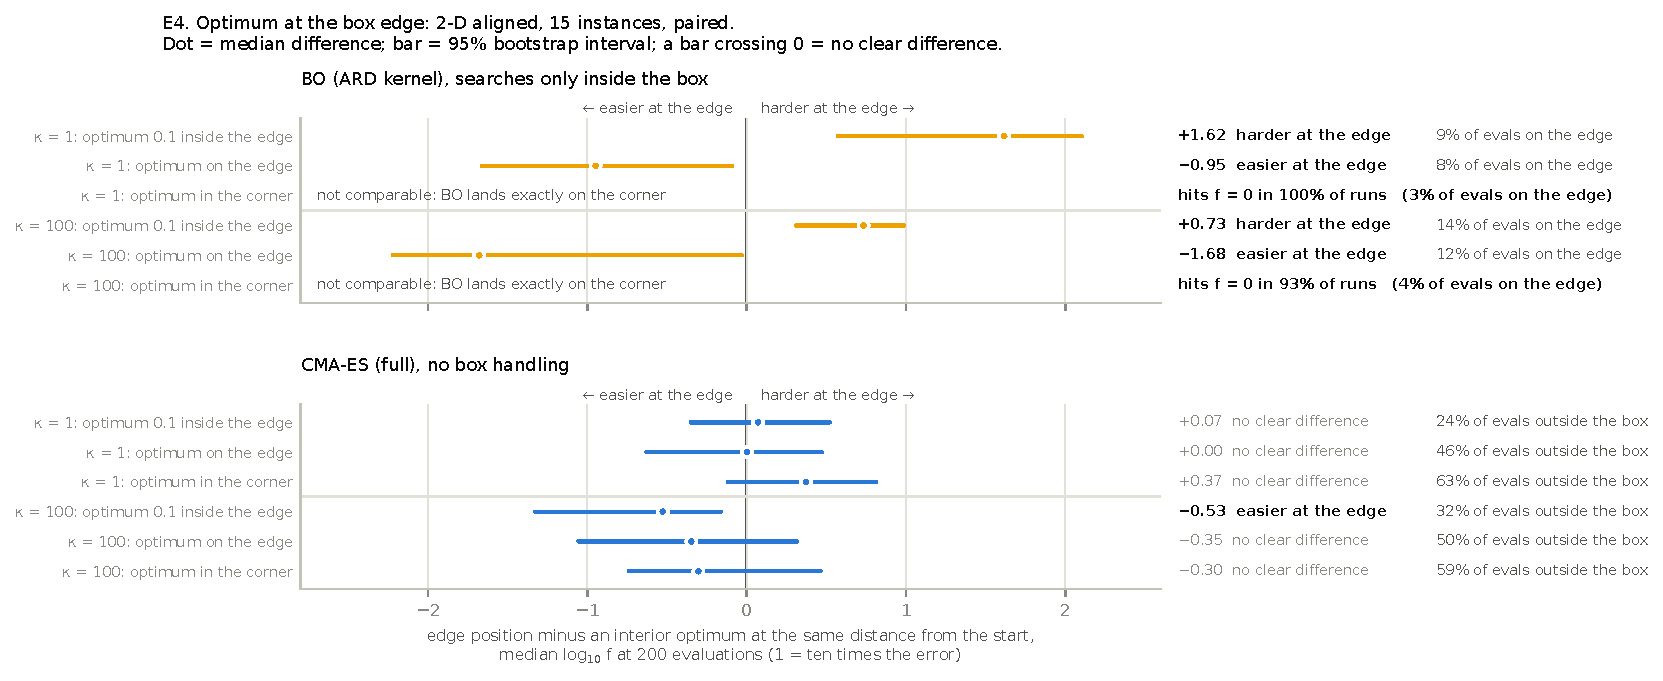
\includegraphics[width=0.95\linewidth]{figures/geom_e4_boundary.pdf}
\caption{Part B, E4. Each edge position minus an interior optimum at the same distance from the start, median
$\log_{10}f$ at 200 evaluations over 15 paired instances; bar = 95\% bootstrap interval. Right: verdict, and the
share of evaluations on the edge (BO) or outside the box (CMA-ES).}
\label{fig:e4}
\end{figure}

\subsection{Under noise, spend the budget on new points and report the model's estimate (E5, E6, E6b)}\label{sec:noise}
At our budget, every evaluation is better spent on a new point than on a repeat, and which point is
reported matters as much as how the budget is spent. We added Gaussian noise $\sigma\in\{0.01,0.1,1\}$ to the aligned
$\kappa=100$ quadratic (200 noisy evaluations, repeats included; 15 instances; every reported point scored on
the noise-free $f$). Against a baseline that evaluates a new point every time, each family tried repeating each
point four times, keeping 40 evaluations to re-check the best five, and, for CMA-ES, a four times larger
population. Each run was read by the lowest reading, the model's estimate (CMA-ES's mean; BO's lowest posterior
mean) and, for the reserve, the best re-checked average (Fig.~\ref{fig:noise}).

Repeating points made the reported point worse in almost every case: by 1.1--3.0 decades for CMA-ES at every
$\sigma$, and by 1.6 and 1.1 decades for BO at $\sigma=0.01$ and 0.1. Averaging four readings halves the noise but
leaves a quarter as many points to search with, which costs more here. Keeping a reserve never helped. The one split that paid was a larger CMA-ES population at $\sigma=1$
($-0.57$ \ci{-0.85}{-0.08}): its mean averages over many points without spending evaluations on repeats.
The same population cost 0.62 decades at $\sigma=0.01$. The cost of repeats shrinks as $\sigma$ grows
(for BO it is no longer significant at $\sigma=1$), so repeats may pay at higher noise; we did not test this.

The reporting rule matters as much as the split. BO's model estimate beats its lowest reading, often a lucky
draw, by 0.30 decades at $\sigma=0.1$ and 1.08 at $\sigma=1$. CMA-ES's mean helps
only with the larger population ($-0.47$ and $-0.33$); with $\lambda=6$ it averages just three points. The
rule must also match the split. With averaged repeats, BO's model estimate was \emph{worse} than its lowest
reading ($+0.89$ \ci{+0.00}{+1.54} at $\sigma=0.01$, borderline). The GP that picks the recommendation learns its
noise level, so it fails as in Section~\ref{sec:stall}: it smooths over its best points. Its error at the lowest
reading was more than three times the gap between the two best readings, and it fitted \emph{more} noise to the
averaged data than to single readings (SD 0.37 against 0.22), although averaging halves the true noise. Without
repeats the same smoothing helps, because a single lowest reading is often a lucky draw. A GP fitted to raw $f$
with the true noise level ($\sigma^2/4$) was never worse than the lowest reading, and was better at
$\sigma=1$ ($-0.50$ \ci{-1.13}{-0.12}; E6b). It changes both the log and the noise, so it does not show which
one mattered. Our prediction that fixing BO's noise would backfire under noise
also failed: fixed noise still beat fitted noise ($-0.41$ \ci{-0.73}{-0.10} at $\sigma=0.01$; E5). With each
family's best settings, BO and CMA-ES end level at every $\sigma$.

These answers hold for one noise distribution, Gaussian of constant size; heavy-tailed noise, noise that grows
with $f$ (as in COCO's noisy suite) or varies across the domain could change the value of repeats, as could other
repeat counts, budgets or dimensions.

\begin{figure}[t]
\centering\includegraphics[width=0.95\linewidth]{figures/geom_e6_noise.pdf}
\caption{Part B, E6. Top: model's estimate minus lowest reading. Bottom: each budget split minus a new point
every evaluation. Dot = median difference in $\log_{10}f$ of the reported point over 15 paired instances;
bar = 95\% bootstrap interval; the verdict on the right is read from whether the bar crosses 0.}
\label{fig:noise}
\end{figure}

\subsection{Predictions against outcomes}
\begin{table}[H]
\centering\footnotesize
\begin{tabular}{p{6.0cm}lp{1.9cm}p{6.0cm}}
\toprule
Prediction (written before the runs) & Exp & Outcome & Evidence \\
\midrule
(i) diagonal CMA-ES pays under rotation & E1 & Held & 0/15 solved at $30^\circ$--$60^\circ$, $\kappa=1{,}000$ \\
(i) BO-ARD pays under rotation (first run) & E2 & Failed & $+0.05$ \ci{-0.53}{+0.63}: BO was stalling \\
(i) BO-ARD pays once BO works & E2, E8, E10 & Held & $+1.06$ to $+2.92$ decades, rotated $\kappa=10^4$ \\
(ii) no penalty on aligned problems & E1, E2, E10 & Held & aligned differences not significant \\
(iii) tilting costs a little when not needed & E10 & Held & aligned $\kappa=100$: ARD box 0.57 better \\
CMA-ES is exactly invariant to monotone maps of $f$ & E3 & Held & 120/120 runs bit-identical \\
BO is nearly invariant to powers of $f$ & E3 & Failed & cube of $f$: $+1.7$ decades \\
fixing BO's noise backfires on noisy problems & E5 & Failed & fixed noise still better, $-0.41$ \\
both CMA-ES variants solve Rosenbrock with 4,000 evaluations & E9 & Failed & diagonal: 0/15 (f8), 4/15 (f9) \\
a locally fitted trust region follows the bend better & E12 & Failed & 1.8--2.0 decades worse; control 2.7 worse \\
\bottomrule
\end{tabular}
\caption{Part B. Selected predictions and how they fared (all 21 in \texttt{geometry/}).}
\end{table}

%=====================================================================
\section{Synthesis: what the two parts establish together}\label{sec:synth}
%=====================================================================
%% AUTHORS: joint section, rewrite together.
\textbf{Shape and scale both decide success, within each family.} Part A shows that a model with the wrong
\emph{scale} fails to find or to refine a narrow basin, and Part B that a model restricted in \emph{shape} fails on
tilted valleys in both families. In neither part does the family alone predict the outcome: diagonal and full
CMA-ES differ by up to 100 percentage points on the same rotated problem, and capped and default BO by 43 successes out of 50
on the same landscape (44 against 1 on fresh seeds).

\textbf{BO's decisive fixes were to the model fit, not the acquisition.} Independently, both parts found BO
failing because its GP was mis-fitted, and both found acquisition changes nearly powerless: in Part A the lengthscale
ran to its bound (capping it took success from 5 to 39/50; $\xi$, LCB and Thompson sampling at most 17/50), in Part B
the fitted noise absorbed the best points (fixing it gained over a decade; LogEI nothing). In both, BO's
results depend on implementation choices that published defaults leave open.

\textbf{CMA-ES adapts shape well but must commit to a scale.} One step size cannot both find a distant basin and refine a
narrow one (Part A), but its covariance follows a rotated valley reliably (Part B); population size and restarts,
which change only how much is sampled, did not move success on the primary landscape.

\textbf{Trade-offs.} BO leads early in both parts and costs roughly $10^5$ times more computation per run; settings
that help on the hard landscape cost on easy ones (the cap on the sphere, tilting on aligned problems); and BO's
boundary preference appears in both parts (edge sampling under large $\xi$; the boundary trap).

\textbf{Limitations.} All headline results are 2-D, so dimension effects are inferred (for CMA-ES) rather than
measured for BO. Each part rests on few landscapes (ellipsoids and Rosenbrock; one primary landscape plus two validation
functions) and 15--50 seeds, which leaves some differences unresolved. BO results reproduce in distribution only: long
BO runs are not bit-repeatable even with one BLAS thread. Some follow-ups were added after seeing results and are
labelled as such; untested mechanisms are stated as hypotheses.

\clearpage
\small
\bibliographystyle{abbrvnat}
\bibliography{references}

\end{document}
